%
%  Scott Percic
%
\documentclass[12pt,fullpage]{article}
\usepackage{fullpage}
\usepackage{psfrag}                                          % LaTeX graphics tool
\usepackage{pslatex}                                         % avoids the default cmr font
\usepackage{graphicx}                                        % graphics package 
\usepackage{epsfig}                                          % figures
\usepackage{hyperref}
\usepackage{color}

\begin{document}

\noindent
{\bf Hyperbolic-secant distribution} (from \color{blue}\url{http://www.math.wm.edu/~leemis/chart/UDR/UDR.html}\color{black})

\noindent
The hyperbolic-secant distribution has probability density function 
$$
f(x) ={\rm sech}(\pi \kern 0.08 em x), \qquad \qquad -\infty<x<\infty,
$$where the hyperbolic-secant function is defined by $${\rm sech}(z)=\frac{2}{e^{\kern 0.08 em z}+e^{-z}}$$ for $-\infty < z < \infty$. The probability density function is illustrated below.
{\begin{figure}[h!]
\begin{center}
\psfrag{labx}{$x$}
\psfrag{labf}{$f(x)$}
\includegraphics[width=3.2in]{HyperbolicsecantPlot.ps}
\end{center}
\end{figure}}\\
The cumulative distribution function on
the support of $X$ is
$$
F(x) = P(X \leq x)= \frac{\pi +2\arctan(\sinh(\pi\, x))}{2\pi} \qquad \qquad -\infty<x<\infty.
$$
The survivor function on the support of $X$ is
$$
S(x) = P(X \geq x) =\frac{\pi - 2\arctan(\sinh(\pi\, x))}{2\pi} \qquad \qquad -\infty<x<\infty.
$$
The hazard function on the support of $X$ is
$$
h(x) = \frac{f(x)}{S(x)} = -\frac{2\pi}{\cosh(\pi \, x)(\pi -2\arctan(\sinh(\pi\, x)))} \qquad \qquad -\infty<x<\infty.
$$
The cumulative hazard function on the support of $X$ is
$$
H(x) = - \ln S(x) = \ln(2) + \ln(\pi) -\ln(\pi-2\arctan(\sinh(\pi \, x))) \qquad -\infty<x<\infty.
$$
The inverse distribution function of $X$ is
$$
F ^ {-1}(u) = \frac{\arcsin(\cot(\pi\, u))}{\pi} \qquad \qquad 0 < u < 1.
$$
The median of $X$ is 0.\\
\\
The moment generating function of $X$ is
$$
M(t) = E\left[ e ^ {\kern 0.08 em tX} \right] = \displaystyle \int_{\kern -0.08 em -\infty}^{\infty} {\rm sech}(\pi \kern 0.08 em x) \qquad \qquad t > 0.
$$
The characteristic function of $X$ is
$$
\phi(t) = E\left[ e ^ {\kern 0.08 em itX} \right] = \displaystyle \int_{\kern -0.08 em -\infty}^{\infty} {\rm sech}(\pi \kern 0.08 em x) \qquad \qquad t > 0.
$$
The population mean, variance, skewness, and kurtosis of $X$ are
$$
E[X] =0 \qquad \qquad 
V[X] = 1 \qquad \qquad 
E\left[ \left( \frac{X - \mu}{\sigma} \right) ^ {\kern -0.08 em 3} \right] = 0 \qquad \qquad 
E\left[ \left( \frac{X - \mu}{\sigma} \right) ^ {\kern -0.08 em 4} \right] = 2.
$$
\vspace{0.1in}

\noindent
{\bf APPL verification:}
The APPL statements
\begin{verbatim}
X := HyperbolicSecantRV();
CDF(X);
SF(X);
HF(X);
CHF(X);
IDF(X);
Mean(X);
Skewness(X);
MGF(X);
\end{verbatim}
verify the cumulative distribution function, survivor function,hazard function, cumulative hazard function, inverse function, population mean, skewness, and moment generating function. APPL fails to verify the population variance and kurtosis.

\end{document}
